% LaTeX Datei f�r Projektarbeiten etc. am MZH

% ------------------------------------------------------------------------------------------
% erlaubt das Anfangen des Draft-Modus und damit Ver�nderungen
% einzustellen
\newif\ifdraft
% Draft-Modus: Arbeitsversion, Bilder werden nur als Rahmen dargestellt
% Vorteil: schnelleres Kompilieren
%\drafttrue % <- daf�r hier die Kommentierung wegnehmen

%-------------------------------------------------------------------------------------------
% folgende Befehle sorgen daf�r, das f�r jede Schrift die richtigen Pakete installiert werden
\newcounter{schrift}
% Schrift ausw�hlen:
% 1 - mathptmx
% 2 - minionpro
% 3 - mathpazo
% 4 - times + computer modern
% 5 - computer modern
\setcounter{schrift}{4} % Hier die entsprechende Zahl setzen !

% ------------------------------------------------------------------------------------------
% ------------------------------------------------------------------------------------------
% Latex - Pr�ambel
% hier werden alle wichtigen Dokumenteinstellungen getroffen, normalerweise m�ssen
% keine �nderungen mehr durchgef�hrt werden.
% Pakete die das Schriftbild, den Satzspiegel oder die R�nder ver�ndern, d�rfen
% nicht hinzugef�gt werden, erst nach Abstimmung mit dem Betreuer.
% n�tzliche Pakete sind willkommen, bitte die Wiki entsprechend aktualisieren
% viele Pakete sind drin, die vielleicht nicht jeder braucht und das Kompilieren verl�ngern
% sollten diese das Layout nicht ver�ndern, k�nnen diese nat�rlich auskommentiert werden.
% ------------------------------------------------------------------------------------------

% ------------------------------------------------------------------------------------------
% Dokumentenklasse definieren:
\ifdraft
    \documentclass[draft, 
                   paper=a4,
                   BCOR5mm,
                   fontsize=12pt, 
                   DIV13, 
                   headsepline, 
                   numbers=noenddot, 
                   %bibtotoc,
                   bibliography = totoc,
                   %version=first,
                   %smallheadings,
                   headings = small,
                   oneside]{scrbook}
\else
    \documentclass[paper=
                   a4,
                   BCOR5mm,
                   fontsize=12pt, 
                   DIV13, 
                   headsepline, 
                   numbers=noenddot, 
                   %bibtotoc,
                   bibliography = totoc, 
                   %version=first,
                   %smallheadings,
                   headings = small,
                   headinclude=true,
                   footinclude=false,
                   fleqn, % formeln links b�ndig
                   oneside]{scrbook}
\fi
% Standard-Koma-Dokument mit
%   Papierformat A4
%   Binderand 5 mm
%   Schrift 12-Punkt
%   Seitenlayout nach DIV, siehe scrguide.pdf text b/h rand oben/innen: 168,00 237,60 19,80 14,00 (ist raus)
%   Linie unter der Kopfzeile
%   Nummern ohne Punkt am Ende
%   Literaturverzeichnis im Inhaltsverzeichnis
%   �berschriften etwas kleiner als standard
%   weitere Informationen zum Koma-Skript: www.komascript.de

%---------------------------------------------------------------
% Basis-Pakete
%---------------------------------------------------------------
\usepackage{ifpdf}		%   Ueberprueft, ob LaTeX oder pdfLaTeX verwendet wird (nur ab MikTeX 2.5)
\usepackage[T1]{fontenc}        %   8-Bit-Fonts
\usepackage{textcomp,latexsym}  %   zusaetzliche Symbole
\usepackage[ansinew]{inputenc}   %   Quelltext ist Latin-1 (d.h. Windows-) kodiert
\usepackage[ngerman]{babel}            %   neue deutsche Rechtschreibung
\usepackage{scrtime}            %   fuer die aktuelle Zeit
%\usepackage{scrdate}            %   fuer das aktuelle Datum
%\usepackage{natbib}             %   Literaturverweise mit (Autor Jahr) nach DIN
%\bibpunct[; ]{[}{]}{,}{a}{}{;}  %   eckige Klammern statt runde bei Zitaten
%\usepackage[T1]{url}            %   Web-Addressen auch mit T1-Encoding
%\urlstyle{tt}                   %   und in tt-Font
%\usepackage[activate=normal]{pdfcprot} % dient dem optischen Randausgleich bei k�rzeren Zeichen wie '-', '.', ',', '!'

\usepackage{color}

\PassOptionsToPackage{x11names}{xcolor}
\usepackage{xcolor}


%---------------------------------------------------------------
% n�tzliche Zusatz-Pakete
%---------------------------------------------------------------
%\usepackage{makeidx}            %   Index (wenn gewuenscht)

\usepackage{setspace}           %   Zeilenabstand setzen. Befehl:
                                %   \begin{spacing{Wert}
                                %   Text
                                %   \end{spacing}
%\usepackage{placeins}           %   das Positionieren von float-Umgebungen bestimmen:
                                %   der Befehl \floatbarrier sorgt daf�r, dass alle vorher eingegebenen
                                %   float-Umgebungen VOR diesem Befehl eingef�gt werden.
                                
%\usepackage{subfig}          %   Bilder gruppieren, mehrere Bilder in einer Umgebung einf�gen
                                %   Bsp.:
                                %   \begin{figure}
                                %   \centering
                                %    \subfloat[Text a]
                                %    {\includegraphics{bild a}}
                                %    \subfloat[text b]
                                %    {\includegraphics{bild b}}
                                %    \caption{Untertitel}
                                %    \label{fig.Beziechnung_subfigure} <- am besten mit fig. dann kann mit \bild{Bezeichnung_figure} referenziert werden
                                %   \end{figure}                                

%\usepackage{textcomp}           %   fuer Trademark und Copyright Zeichen
                                %   z.B \texttrademark, \textregistered, \texteuro etc.

\usepackage{tabularx}           %   erweiterte Funktionen f�r Tabellen

\usepackage{longtable}          %   Longtable-Package f�r Tabellen die l�nger als eine DIN-A4-Seite sind

\usepackage{colortbl}						%		farbige Tabellenzeilen

\usepackage{nicefrac}           %   Schr�ge Bruchstriche \nicefrac{Nenner}{Z�hler}

%\usepackage{numprint}           %   Zahlen mit Einheiten n�her an der Zahl/kein Umbruch und 1 000er Format \numprint[Einheit]{Zahl}

%\usepackage{mathcomp}           %   f�r \tcdegree (� Gradzeichen bei numprint) \numprint[\tcdegree]{180} f�r 180�

%\usepackage{hhline}             %   hhline-Package
                                %   Fuer komplexe Linienzuege in Tabellen \hhline{}
                                %   = Spalte mit doppelter Linie      | vertikale Linie die horizontale schneidet
                                %   - Spalte mit einfacher Linie      : vertikale Linie die von horizantaler unterbrochen ist
                                %   ~ Spalte ohne Linie               # doppelte horiz. geschnitten mit doppelter vert. Linie
                                %   t oberer Teil ->                  b unterer Teil einer doppelten Linie

%\usepackage[active]{srcltx}     %   bei verwendung v. \includeonly spring winedt jetzt bei fehlern an die richtige stelle

\usepackage{flafter}            %   Ein float-Objekt immer erst NACH seiner Definition platzieren

\usepackage{ifthen}             %   definiert \ifthenelse{}{}{}

%\usepackage{path}               %   dateinamen und pfade darstellen

%\usepackage{pdfsync}						%   Synchronisation mit SumatraPDF <<-- geht auch ohne

\usepackage{booktabs}

%% Eigene Pakete

\usepackage{scrhack} % L�scht Warnungen von Packages wie hyperref, listings
\usepackage[ locale = DE,            % deutsch
            load-configurations=abbreviations, % zus�tzliche Einheiten siehe manual
            per-mode=symbol,%-or-fraction,
            separate-uncertainty% 
            ]
            {siunitx}								% SI-Einheiten  

            
\usepackage{multirow}               % zwei Zeilen kombinieren (wie multicolumn)
\usepackage[babel]{microtype}       % schickeres Schriftbild -> aber l�ngeres Kompilieren

\usepackage{blindtext}							% sinnlosen text einbauen
\usepackage{subfigure}

\usepackage{newunicodechar}
%\newunicodechar{ }{~}

%\DeclareUnicodeCharacter{00A0}{~}


%%

%---------------------------------------------------------------
% Grafik-Paket f�r eps bzw. pdf
%---------------------------------------------------------------
% �berpr�ft ob Latex oder PDFLatex ausgef�hrt wird, dementsprechend werden pdf/jpg oder eps Bilder eingef�gt
% sollen dvi oder pdf Dokumente erstellt werden m�ssen alle Bilder in beiden Formaten vorliegen
% hierf�r gibt es Tools wie epstopdf oder jpgtoeps
 \ifdraft
    \usepackage[draft]{graphicx}
\else
    \ifpdf
        \usepackage{graphicx}
        \usepackage{pgfplots} % pgfplots zum plotten in LaTeX
    \else
        \usepackage[final]{graphicx}
    \fi
\fi
% von wo sollen die Grafiken kommen?
\graphicspath{{./fotos/}{./skizzen/}{./zeichnungen/}{./plots/}}

%Einstellungen f�r pgfplots
\pgfplotsset{compat=1.3,
	%enlargelimits=auto,
	tick label style={font=\small,/pgf/number format/use comma}, %Komma nutzen in allen Axen
	%axis x line=center, %alle x-Achsen center
	%axis y line=center, %alle y-achsen center
	%every axis x label/.style={at={(current axis.right of origin)},anchor=west}, % achsenbeschriftung bei allen x-achsen rechts
	%every axis y label/.style={at={(current axis.above origin)},anchor=south},   % achsenbeschriftung bei allen y-achsen oben
	%every x tick scale label/.style={at={(current axis.right of origin)},anchor=north,yshift=-0.5em}, %positionierung des scale faktors ge�ndert
	every axis legend/.append style={at={(0.5,1.03)},anchor=south,nodes=right,font=\small}, % Legende �ber der Grafik, schriftgr��e small
	label style={font=\small} % label schriftgr��e small
}
\newlength\tikzwidth
\setlength{\tikzwidth}{0.7\textwidth}
\definecolor{mycolor1}{rgb}{0,0.5,0}

\ifpdf
 \ifdraft
    \usepackage[draft]{pdfpages}%   externe PDF Seiten einbinden nur bei PDF-Latex m�glich
    \else
    \usepackage[final]{pdfpages}%   externe PDF Seiten einbinden nur bei PDF-Latex m�glich
 \fi                            %   Befehl: \includepdf{PDF-Datei} soll die Datei im Querformat angezeigt werden
    \else
\fi                             %   \includepdf[landscape=true]{PDF-Datei}

%---------------------------------------------------------------
% Debug-Ausgabe der Labels und References
%---------------------------------------------------------------
\ifdraft
  \usepackage{showkeys} % Label werden im Draft Modus im Text angezeigt
\fi

%---------------------------------------------------------------
% Abweichende PostScript-Schriftarten
% werden in der main Datei ausgew�hlt, hier nichts �ndern
%---------------------------------------------------------------
\ifthenelse{\equal{ 1 }{ \value{schrift} }}
    {
    \usepackage{mathptmx}          %   Times als Hauptschriftart, keine mathematische Fettschrift
    \usepackage{amssymb}
    \usepackage{amsbsy}
    \usepackage{amsmath}
    \usepackage{amsfonts}
    \usepackage{amstext}
    \renewcommand{\boldsymbol}[1]{\mathbf{#1}} % nur bei mathptmx !
                                               % damit boldsymbol wenigstens fette aufrechte Buchstaben macht
    }{}
\ifthenelse{\equal{ 2 }{ \value{schrift} }}
    {
    \usepackage[lf, minionint]{MinionPro} %   OpenType von Adobe, mathematische Fettschrift vorhanden, Schrift ist
                                %   ist im Standard-LaTeX nicht installiert.
                                %   Ist ein wenig Aufwand das Ganze zu installieren, Matthias Dagen fragen
    }{}
\ifthenelse{\equal{ 3 }{ \value{schrift} }}
    {
    \usepackage{mathpazo}          %   nette Buchschrift aber sehr gross, mathematische Fettschrift vorhanden
    \usepackage{amssymb}
    \usepackage{amsbsy}
    \usepackage{amsmath}
    \usepackage{amsfonts}
    \usepackage{amstext}
    }{}
\ifthenelse{\equal{ 4 }{ \value{schrift} }}
    {
    \usepackage{times}
    \usepackage{amssymb}
    \usepackage{amsbsy}
    \usepackage{amsmath}
    \usepackage{amsfonts}
    \usepackage{amstext}
    }{}
\ifthenelse{\equal{ 5 }{ \value{schrift} }}
    {
    \usepackage{amssymb}
    \usepackage{amsbsy}
    \usepackage{amsmath}
    \usepackage{amsfonts}
    \usepackage{amstext}
    \usepackage{lmodern}
    }{}
\usepackage[scaled=.92]{helvet} %   11pt Helvetica f�r �berschriften etc. etwas kleiner da, Helvetica an sich gr��er ist
%\usepackage{courier}            %   Courier bei \texttt
%\usepackage{upgreek}            %   Aufrechte griechische Buchstaben

% ------------------------------------------------------------------------------------------
% Bild- und Tabellentitel FETT
% ------------------------------------------------------------------------------------------
%\def\figurename{\bfseries Bild}
%\def\tablename{\bfseries Tabelle}

%%Andere Beschreibung von figure
\addto\captionsngerman{
	\renewcommand{\figurename}{\bfseries Bild}%%Andere Beschreibung von figure
	\renewcommand{\listfigurename}{Bildverzeichnis}
	\renewcommand{\tablename}{\bfseries Tabelle}
}

%---------------------------------------------------------------
% Quelltexte formatieren
%---------------------------------------------------------------
\usepackage{listings}


%\lstloadlanguages{
		%C,
		%C++,
		%XML
%}

\lstset{
		language=XML,
		basicstyle=\footnotesize\ttfamily, % Standardschrift
		numbers=left,               % Ort der Zeilennummern
		numberstyle=\tiny,          % Stil der Zeilennummern
		numbersep=5pt,              % Abstand der Nummern zum Text
		tabsize=2,                  % Groesse von Tabs
		extendedchars=true,         %
		breaklines=true,            % Zeilen werden Umgebrochen        
		keywordstyle=\color{Red2},
		frame= b,         
		stringstyle=\color{Purple2}\ttfamily, % Farbe der String
		showspaces=false,           % Leerzeichen anzeigen ?
		showtabs=false,             % Tabs anzeigen ?
		xleftmargin=17.5pt,
		framexleftmargin=17pt,
		framexrightmargin=5pt,
		framexbottommargin=4pt,
		linewidth= \dimexpr\textwidth-2\fboxsep-2\fboxrule,
		comment=[l]{\#},
		morecomment=[s]{<!--}{-->},
		commentstyle=\color{Green4},
		%backgroundcolor=\color{grey},
		showstringspaces=false,      % Leerzeichen in Strings anzeigen ?        
		morekeywords={__global__, name, pkg, args, type, from, to, textfile, respawn, value, output, radius, ixx, ixy, ixz, iyy, iyz, xyz, rpy, reference},  % CUDA specific keywords
		aboveskip = 18pt, 
		belowskip = 18pt
}

\usepackage{caption}
\DeclareCaptionFont{white}{\color{white}}
\DeclareCaptionFormat{listing}{\colorbox{darkgray}{\parbox{\dimexpr\textwidth-2\fboxsep-2\fboxrule}{\hspace{15pt}#1#2#3}}}
\captionsetup[lstlisting]{format=listing,labelfont=white,textfont=white, singlelinecheck=false, margin=0pt, font={bf,footnotesize}}

%---------------------------------------------------------------
% ein paar L�ngen einstellen
%---------------------------------------------------------------
%\setlength{\parskip}{1ex plus0.5ex minus0.2ex} % Absatzabstand etwas gr��er
\setlength{\itemsep}{0ex plus0.2ex}            % Abstand zweier Listenelemente kleiner
\setlength{\parindent}{0ex}                     % kein Absatzeinzug
\setlength{\belowcaptionskip}{0.4cm}            % Abstand caption - Tabelle gr��er
\setlength{\abovecaptionskip}{0.4cm}            % Abstand caption - Tabelle gr��er

%---------------------------------------------------------------
% Kopf- und Fusszeilen
%---------------------------------------------------------------
\usepackage[plainheadsepline,  % linie zw. kopf und text auch bei seitenstil "plain"
           %headexclude,       % kopfzeile geh�rt nicht zum textk�rper
           %footexclude        % fusszeile geh�rt nicht zum textk�rper
          ]       
           {scrpage2}
\pagestyle{scrheadings}
\clearscrheadfoot              % voreinstellungen loeschen
\ihead{\normalfont\headmark}   % kolumnentitel innen
\ohead[\pagemark]{\pagemark}   % seitenzahl aussen

%---------------------------------------------------------------
% Nummerierungs-Tiefe des Inhaltsverzeichnis und der Abschnitte einstellen
%---------------------------------------------------------------
\setcounter{secnumdepth}{2} \setcounter{tocdepth}{2}

%---------------------------------------------------------------
% Abk�rzungsverzeichnis
%---------------------------------------------------------------
% mit dem Befehl \nomenclature[l/g/a]{Abk�rzung}{Bezeichnung} kann direkt im Code die Abk�rzung eingef�gt werden
% das Paket sortiert diese und f�gt sie mit dem Befehl \printnomenclature ein
% l, g, oder a steht dabei f�r die Gruppierung Lateinische bzw. Griechische Buchstaben, Abk�rzungen
% Nach Einf�gen neuer Abk�rzungen muss folgender Befehl in der Eingabeaufforderung im Tex-Verzeichnis eingegeben werden:
% -> vorher einmal kompilieren
% -> makeindex main.nlo -s nomencl.ist -o main.nls
% -> nochmal kompilieren
%\makeindex
\usepackage{nomencl}
% \let\abbrev\nomenclature
\renewcommand{\nomname}{Abk�rzungsverzeichnis}
\setlength{\nomlabelwidth}{.25\hsize}
\renewcommand{\nomlabel}[1]{#1 \hfill}
\setlength{\nomitemsep}{-\parsep}

\renewcommand{\nomgroup}[1]{%
	\ifthenelse{\equal{#1}{L}}{\item[\textbf{Lateinische Buchstaben}]}
	{%
		\ifthenelse{\equal{#1}{G}}{\item[\textbf{Griechische Buchstaben}]}
		{%
			\ifthenelse{\equal{#1}{A}}{\item[\textbf{Abk�rzungen}]}
			{
				\ifthenelse{\equal{#1}{K}}{\item[\textbf{Koordinatensysteme}]}{}
			}
		}
	}
}

\makenomenclature

%---------------------------------------------------------------
% Hyperlinks f�r pdfTeX
%---------------------------------------------------------------
\ifpdf
    % hier stehen befehle, die nur f�r pdftex gelten
    \usepackage[pdfpagelabels,  % logische (z.b. auch roemische) seitenzahlen
                bookmarks,       % Bookmarks f�r die einzelnen Abschnitte
                pdftex
                ]{hyperref}
    \hypersetup{
    %   colorlinks,  % Links mit farbigem Text
        pdfborder   = 0 0 0,
        plainpages  = false,
        bookmarksnumbered = true,
    %   bookmarksopen
    }
\else
    % hier stehen befehle, die nur f�r latex gelten
    \usepackage{hyperref} % hier ohne colorlinks und pdf-krams
\fi

%extra inhaltsverzeichnisse m�glich
\usepackage[nohints]{minitoc}     
\renewcommand{\mtctitle}{Anhangsverzeichnis} 				% Name �ndern            
\renewcommand{\mtifont}{\large\bfseries\sffamily}		% Titel font �ndern
\renewcommand{\mtcSfont}{\rm}												% Section eintr�ge normal
\mtcsetrules{minitoc}{off}													% Linien ausmachen

%---------------------------------------------------------------
% SVGs einf�gen
%---------------------------------------------------------------
%% SVG to TeX
% from InkscapePDFLaTeX.pdf
% by Johan Engelen, 2010
% Information: 
% http://tug.ctan.org/tex-archive/info/svg-inkscape
% -shell-escape muss im Ausgabeprofil stehen
% inkscape.exe muss im Path-Folder sein

% Funktion zum ueberpruefen auf Aenderung
\newcommand{\executeiffilenewer}[3]{%
                \ifnum\pdfstrcmp{\pdffilemoddate{#1}}%
                {\pdffilemoddate{#2}}>0%
                {\immediate\write18{#3}}\fi%
}
% Wenn Aenderung dann TeX-Export ausfuehren und einbinden
%\newcommand{\includesvg}[1]{%
                %\executeiffilenewer{#1.svg}{#1.pdf}%
                %{inkscape -z -C --file=#1.svg %
                %--export-pdf=#1.pdf --export-latex}%
                %\input{#1.pdf_tex}%
%}

%% Include svg mit Text aus textext plugin
% text wird im svg mit textext hinzugef�gt.
% falls �nderungen im .svg gefunden werden, wird das Bild 
% neu exportiert und eingef�gt.
% \includesvg{ordner/file} /ohne endung
\newcommand{\includesvg}[4][]{
			\executeiffilenewer{#3.svg}{#3.pdf}
			{inkscape -z -D --file=#3.svg
			--export-pdf=#3.pdf}
			\begin{figure}[#2]
				\centering
				\includegraphics[#1]{#3}
				\caption{#4} \label{fig.#3}
				\vspace*{-3mm}
			\end{figure}
}

\newcommand{\includesinglesvg}[2][]{
			\executeiffilenewer{#2.svg}{#2.pdf}
			{inkscape -z -D --file=#2.svg
			--export-pdf=#2.pdf}
			\includegraphics[#1]{#2}
}

\usepackage[right]{eurosym}

                           % Pr�ambel zur Dokumentenformatierung einf�gen
                                            % braucht nicht zu ver�ndert werden, stehen aber n�tzliche
                                            % Hinweise drin

%---------------------------------------------------------------
% Trennmuster fuer Ausnahmef�lle
%---------------------------------------------------------------
\hyphenation{} % z.B. \hypenation{Trenn-text}
\hyphenation{Kraft-ein-wirk-ung}
\hyphenation{ein-ge-spannt}
\hyphenation{Coch-lea-im-plan-ta-te}
\hyphenation{Deh-nungs-mess-streifen}

%---------------------------------------------------------------
% Dokumentenanfang:
%---------------------------------------------------------------
% Einstellungen f�r PDF-Latex:
% Hier Titel etc. eintragen, dann wird es in den Dokumenteneigenschaften vom PDF richtig angezeigt
\ifpdf
    \hypersetup{
    %   colorlinks,  % Links mit farbigem Text
        pdftitle    = {Nichtlineare Zustandsbeobachtung mit bildbasierter Validierung am inversen Doppelpendel},
        pdfsubject  = {Studienarbeit},
        pdfauthor   = {Andreas Serov},
        pdfkeywords = {Zustandsbeobachtung, Doppelpendel}
        }
\else
\fi

%\usepackage[utf8]{inputenc}					% umlaute
%\usepackage[ansinew]{inputenc}				% umlaute
\usepackage{befehle}                        % eigene Befehle wie:
                                            % \zB\,
                                            % \abbildung{Position h,b,t,p}{Dateiname ohne Endung}{Caption}
                                            % \bild{Dateiname}, referenziert gem�� ...Bild x.xx...
                                            % einfach mal nachschauen was so drin ist und eigene Befehle f�r
                                            % wiederholende Sachen definieren

%\includeonly{ergebnisse}                   % wenn nur ein Kapitel kompilliert werden soll
                                            % geht schneller wenn man nur das Layout des Kapitels sehen will

%\entwurf                                   % Entwurfsdatum auf jede Seite setzen,
                                            % nicht vergessen beim Druck rauszunehmen
%\setlength\overfullrule{5pt}                % Overfull boxes werden angezeigt
%\setlength\underfullrule{5pt} 

% Seitenspiegel neu berechnen
\typearea[current]{last}
%\typearea{last}
\begin{document}                            % Dokumentenanfang
\dominitoc
\begin{spacing}{1.15}                       % Zeilenabstand auf 1,15 fach stellen, ist nicht so eng aber
                                            % auch nicht so eine Seitenschinderei wie 1,5-fach
%    \frontmatter                            % mit kleinen r�mischen Seitenzahlen beginnen f�r class scrbook
%    %\pagenumbering{roman}                  % das gleiche f�crartcl
%    \setcounter{page}{0}
%    \pdfbookmark[0]{Titel}{tit}             % damit der Titel auch im Acrobat angezeigt wird
%		\begin{titlepage}
\begin{spacing}{2}

\begin{flushright} %rechtsb�ndig (Anfang)
	\vspace*{-20mm}
	
\includegraphics[width=\textwidth]{skizzen/CoverLogos}
	%
\includegraphics[width=\textwidth]{skizzen/CoverLogos_MZH}
\end{flushright} %rechtsb�ndig (Anfang)

% der Titel der Arbeit:
\vspace{38mm} {\centering {{\LARGE{Nichtlineare Zustandsbeobachtung mit bildbasierter Validierung am inversen Doppelpendel}}}

\vfill
% hier kommt ne h�bsche Grafik hin:
%\includegraphics[width = 80mm]{youBot}


\vfill }
\end{spacing}
\begin{spacing}{1}
\begin{tabular}{l}
 \Large{Studienarbeit S-03/17-608}
\end{tabular}

\vspace{5mm}

\begin{tabular}{l}
\large{Andreas Serov}\\
\large{Matrikelnummer 2871560}
\end{tabular}

\vspace{5mm}

\begin{tabular}{l}
\large{Hannover, M�rz 2017}
\end{tabular}


\vspace{5mm}
{\large
\begin{tabular}{l l}
Erstpr�fer  & Prof. Dr.-Ing. T. Ortmaier\\
%Zweitpr�fer & Prof. Dr.-Ing. x\\
Betreuer    & M. Sc. Steffen Bosselmann\\
\end{tabular}
}
\afterpage{\blankpage}
\end{spacing}
\end{titlepage}


% --------------------------------------------------
% hier folgt die aufgabenstellung


%\includepdf{pdfs/empty}
%\includepdf{pdfs/AufgabenstellungTeil1}
%\includepdf{pdfs/AufgabenstellungTeil2}

% --------------------------------------------------
% Erkl�rung

\noindent Ich versichere, dass ich diese Studienarbeit selbstst�ndig
verfasst und keine anderen als die angegebenen Hilfsmittel verwendet
habe.

\vspace{25mm}

\noindent Hannover, 28. M�rz 2017
\newpage

%    \clearpage
%    \pdfbookmark[0]{\contentsname}{toc}
%    %\setcounter{page}{1}
%    \tableofcontents                        % Inhaltsverzeichnis
%    \listoffigures
%    \listoftables
%    \printnomenclature                      % Formelverzeichnis einbinden
%    \mainmatter                             % der eigentliche Tex
%		%\input{abkuerzungen}                    % Abk�rzungen im Text, z.B. CI = Cochleaimplantat
%		%%Doppelpendel
\nomenclature[a11]{$ \ell_1 $}{L�nge des inneren Pendels}
\nomenclature[a12]{$ \ell_2 $}{L�nge des �u�eren Pendels}
\nomenclature[a17]{$ M_{\mathrm{Motor}} $ }{Antriebsmoment des Motors}
\nomenclature[a05]{$ F_{\mathrm{a}} $}{Antriebskraft des Wagens}
\nomenclature[a06]{$ F_{\mathrm{r}} $}{Reibkraft zwischen Wagen und Linearf�hrung}
\nomenclature[a23]{$ x $}{Wagenposition}
\nomenclature[a]{$ \varphi_1 $}{Winkel des inneren Pendels}
\nomenclature[a01]{$ \varphi_2 $}{Winkel des �u�eren Pendels}
\nomenclature[a14]{$ m_1 $}{Masse des inneren Pendels}
\nomenclature[a15]{$ m_2 $}{Masse des �u�eren Pendels}
\nomenclature[a16]{$ m_3 $}{Masse des Gelenks}
\nomenclature[a13]{$ m_0 $}{Masse des Wagens}
\nomenclature[a10]{$ L $}{Lagrange-Funktion}
\nomenclature[a18]{$ \bm{q} $}{Vektor der generalisierten Koordinaten}
\nomenclature[a19]{$ \bm{Q}_{\mathrm{n.k.}} $}{Nichtkonservative Kr�fte}
\nomenclature[a08]{$ J^\mathrm{S}_1 $}{Massentr�gheitsmoment des inneren Pendels um den Schwerpunkt}
\nomenclature[a09]{$ J^\mathrm{S}_2 $}{Massentr�gheitsmoment des �u�eren Pendels um den Schwerpunkt}
\nomenclature[a20]{$ T $}{Kinetische Energie}
\nomenclature[a21]{$ U $}{Potentielle Energie}
\nomenclature[a22]{$ v $}{Schwerpunktsgeschwindigkeit}
\nomenclature[a07]{$ g $}{Erdbeschleunigung}
\nomenclature[a03]{$ d_1 $}{D�mpfungskonstante des inneren Pendels}
\nomenclature[a04]{$ d_2 $}{D�mpfungskonstante des �u�eren Pendels}

%Zustandsregelung
\nomenclature[b13]{$ \bm{x}(t) $}{Zustandsvektor}
\nomenclature[b10]{$ u(t) $}{Eingangsgr��e}
\nomenclature[b15]{$ y(t) $}{Ausgangsvektor}
\nomenclature[b]{$ \bm{A} $}{Systemmatrix}
\nomenclature[b02]{$ \bm{b} $}{Steuervektor}
\nomenclature[b03]{$ \bm{C} $}{Beobachtungsmatrix}
\nomenclature[b14]{$ \bm{x}_0 $}{Anfangszustand}
\nomenclature[b09]{$ \bm{S}_\mathrm{S} $}{Steuerbarkeitsmatrix}
\nomenclature[b05]{$ \bm{k}^\mathrm{T} $}{R�ckf�hrvektor}
\nomenclature[b11]{$ V $}{Vorfilter der F�hrungsgr��e}
\nomenclature[b12]{$ w(t) $}{F�hrungsgr��e}
\nomenclature[b01]{$ \tilde{\bm{A}} $}{Systemmatrix des geschlossenen Kreises}
\nomenclature[b04]{$ J $}{G�tefunktional}
\nomenclature[b07]{$ \bm{Q}_{\mathrm{LQ}} $}{Wichtungsmatrix des Zustandsvektors}
\nomenclature[b08]{$ R_{\mathrm{LQ}} $}{Wichtungsfaktor der Eingangsgr��e}
\nomenclature[b06]{$ \bm{P} $}{L�sung der Matrix-Ricattigleichung}

%Nichtlineare Zustandsbeobachtung
\nomenclature[c12]{$ \hat{\bm{x}} $}{Gesch�tzter Zustandsvektor}
\nomenclature[c08]{$ \bm{S}_\mathrm{B} $}{Lineare Beobachtbarkeitsmatrix}
\nomenclature[c09]{$ \bm{S}_{\mathrm{B},\mathrm{nl}}$}{Nichtlineare Beobachtbarkeitsmatrix}
\nomenclature[c11]{$ \bm{w}_k $}{Vektor des Prozessrauschens}
\nomenclature[c10]{$ \bm{v}_k $}{Vektor des Messrauschens}
\nomenclature[c06]{$ \bm{Q}_{\mathrm{EKF}} $}{Matrix des Prozessrauschens}
\nomenclature[c07]{$ \bm{R}_{\mathrm{EKF}} $}{Matrix des Messrauschens}
\nomenclature[c05]{$ \bm{P}_k$}{Matrix der Fehlerkovarianz}
\nomenclature[c04]{$ \bm{P}_0$}{Initiale Fehlerkovarianz}
\nomenclature[c03]{$ \bm{K}_k$}{Kalmanverst�rkung}
\nomenclature[c02]{$ e $}{Fehler der Zustandssch�tzung}
\nomenclature[c13]{$ \ddot{x}(t) $}{Wagenbeschleunigung}
\nomenclature[c14]{$ \ddot{x}_{\mathrm{max}} $}{Amplitude der Wagenbeschleunigung}
\nomenclature[c01]{$ \omega $}{Kreisfrequenz}
\nomenclature[c15]{$ \Delta\ddot{x} $}{Phasenversatz}

%Beobachtervalidierung
\nomenclature[d10]{$ \bm{c}_\mathrm{r} $}{Schwerpunkt des roten Farbmarkers}
\nomenclature[d11]{$ \bm{c}_\mathrm{g} $}{Schwerpunkt des gr�nen Farbmarkers}
\nomenclature[d12]{$ \bm{c}_\mathrm{b} $}{Schwerpunkt des blauen Farbmarkers}
\nomenclature[d03]{$ \varphi_{1,\mathrm{B}} $}{Bildbasierter innerer Pendelwinkel}
\nomenclature[d04]{$ \varphi_{2,\mathrm{B}} $}{Bildbasierter �u�erer Pendelwinkel}
\nomenclature[d01]{$ \alpha_1 $}{innerer Pendelwinkel im Bildkoordinatensystem}
\nomenclature[d02]{$ \alpha_2 $}{�u�erer Pendelwinkel im Bildkoordinatensystem}
\nomenclature[d15]{$ \mathrm{KS}_\mathrm{B} $}{Bildkoordinatensystem}
\nomenclature[d06]{$ \bm{B} $}{RGB-Einzelbild}
\nomenclature[d07]{$ \bm{B}^\mathrm{r} $}{Einzelbild des roten Farbkanals}
\nomenclature[d08]{$ \bm{B}^\mathrm{g} $}{Einzelbild des gr�nen Farbkanals}
\nomenclature[d09]{$ \bm{B}^\mathrm{b} $}{Einzelbild des blauen Farbkanals}
\nomenclature[d13]{$ \bm{G}^\mathrm{r} $}{Einzelbild in Graustufen}
\nomenclature[d14]{$ I $}{Intensit�tsschwellwert}
\nomenclature[d16]{$ \bm{SW} $}{Bin�rmaske eines Einzelbilds}
\nomenclature[d05]{$ A $}{Fl�che eines Bildobjekts}
\nomenclature[d17]{$ u_\mathrm{S} $}{Schwerpunktkoordinate der $ u $-Achse}
\nomenclature[d18]{$ v_\mathrm{S} $}{Schwerpunktkoordinate der $ v $-Achse}

                       % Mathematische Variablen
%    \chapter{Einleitung}

Die Abk�rzung etc.\nomenclature{etc.}{et cetera} steht im Abk�rzungsverzeichnis. 

%\abbildung[width=60 mm]{htb}{PR2-1}{Beispiel f�r ein einzelnes Bild}										% die einzelnen Kapitel einbinden
%	%\chapter{Stand der Technik}


Das inverse Doppelpendel stellt ein inh�rent instabiles System dar. Es wird in diversen Arbeiten als Ma�stab f�r unter unterschiedliche Regelungs- und Beobachterkonzepte verwendet. 

%\begin{equation}
%sljdsjuhd = luhsdfiuhsf+ spidhfos
%\end{equation}


%	\chapter{Robotersysteme}


Ein bis zwei  zur Einleitung des Kapitels...

%\begin{equation}
%sljdsjuhd = luhsdfiuhsf+ spidhfos
%\end{equation}


\section{PR2}

Der PR2 (Willow Garage Inc., Menlo Park, USA) ist ein \textbf{\textit{menschen�hnlicher} }Serviceroboter, der seinen Dienst in Wohnr�umen verrichten soll und derzeit im sogenannten PR2 Beta-Programm von elf Forschungseinrichtungen �ber einen Zeitraum von zwei Jahren getestet wird \cite{WillowGarage2010}.\\

\begin{figure}[!ht]
	\begin{center}
	\subfigure[]{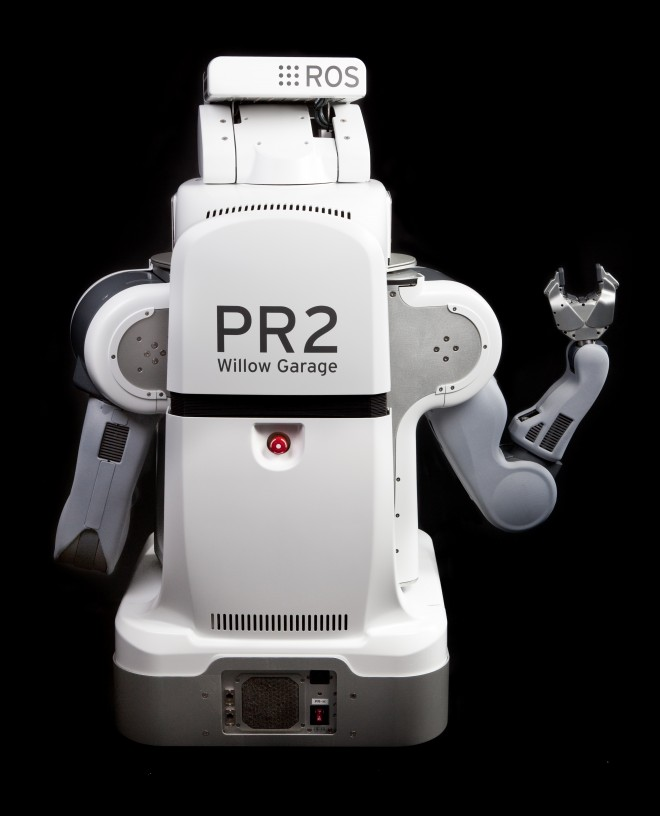
\includegraphics[height=45mm]{PR2-1}}
	\hspace{5mm}
	\subfigure[]{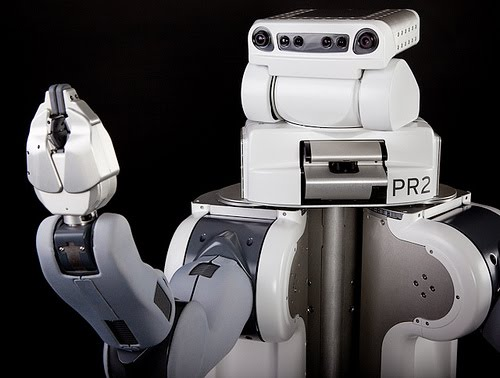
\includegraphics[height=45mm]{PR2-2}}
	\hspace{5mm}
	\subfigure[]{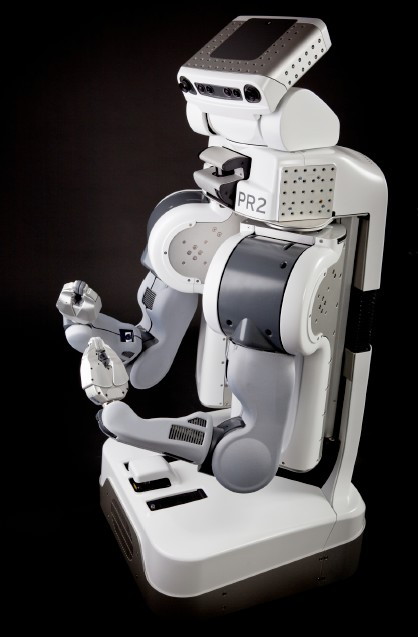
\includegraphics[height=45mm]{PR2-3}}
	\caption{PR2-Roboter (Quelle: Willow Garage)}
	\label{fig.PR2}
	\end{center}
	\vspace*{-8mm}
\end{figure}




Ausgestattet ist der PR2 mit zwei Armen, die jeweils sieben Freiheitsgrade haben und an deren Enden ein Greifer montiert ist, siehe \bild{PR2}. Die Sensorik des Armes besteht aus einer Kamera am Unterarm und Druck- sowie Beschleunigungssensoren am Greifer. Die Nutzlast eines Arms ist mit \SI{1,8}{\kilo\gram} ausgewiesen. Weiterhin verf�gt der Roboter �ber einen dreh- und schwenkbaren Kopf, in dem eine 5-Megapixel Farbkamera, ein LED-Texturprojektor und zwei Stereokameras integriert sind, wobei eine Kamera f�r die Fernsicht und die andere f�r die Objektmanipulation genutzt wird. Unterhalb des Kopfes ist ein schwenkbarer Laserscanner und ein Inertialsensor verbaut. Die Position des Oberk�rpers l�sst sich in der H�he zwischen \SI{1330}{\milli\meter} und \SI{1645}{\milli\meter} (Gesamth�he) variieren. Angetrieben wird die omnidirektionale Basis von vier gelenkten R�dern, die eine maximale Geschwindigkeit von \SI{3,6}{\kilo\meter\per\hour} erm�glichen. Die quadratische Basis hat eine Kantenl�nge von \SI{668}{\milli\meter}. Als Recheneinheit stehen zwei Server zur Verf�gung, die jeweils auf acht CPU-Kernen rechnen und dabei auf 24\,GB Arbeitsspeicher zugreifen k�nnen. Als Betriebssystem wird Ubuntu verwendet, auf dem das Robot Operating System, kurz ROS, die Grundlage f�r die Datenverarbeitung bildet. Da ROS innerhalb dieser Arbeit ebenfalls zum Einsatz kommt, wird dieses in \Sec{IntroductionROS} vorgestellt und an den entsprechenden Stellen weiter erl�utert. Die Kosten f�r einen PR2-Roboter belaufen sich derzeit auf etwa \SI{400.000}{US-Dollar}\footnotemark. Mit Hilfe des PR2 wurden von den zuvor erw�hnten Beta-Testern Szenarien bew�ltigt, die innerhalb des menschlichen Wohnraumes auftreten k�nnen. An der TU M�nchen hat ein PR2-Roboter beispielsweise zusammen mit einem anderen Robotersystem einen Pfannkuchen gebacken \cite{TUM2011}.
\footnotetext{Der angegebene Preis wurde am 16.08.2011 der Website http://www.willowgarage.com/pages/pr2/order entnommen und versteht sich exklusive Steuern und Versandkosten.}

\section{Technische Daten der youBot-Plattform}

\begin{table}[ht]
	\centering
	\caption{Technische Daten der youBot Plattform}\label{tab.TechSpecYouBotBase}
	\vspace*{-3mm}
	\begin{longtable}[ht]{|l|c|r|}\hline
		\rowcolor{Snow2}
		Bezeichnung						& Formelzeichen	& \\ \hline
		Gesamtl�nge 					&			& \SI{530}{\milli\meter}				\\ \hline
		Gesamtbreite 					&  		& \SI{350}{\milli\meter}				\\ \hline
		H�he									&  		& \SI{106}{\milli\meter}				\\ \hline
		Radstand							& $l$	& \SI{470}{\milli\meter}				\\
		\hline
	\end{longtable} 
	\vspace*{-3mm}
\end{table}


\begin{lstlisting}[label=source.launchHokuyo,caption=Launchfile zum Start der hokuyo\_node]
<!-- launch hokuyo node -->
<node pkg="hokuyo_node" type="hokuyo_node" name="hokuyo_node" output="screen">
	<param name="port" value="/dev/ttyACM0"/>
	<param name="frame_id" value="/base_laser_front_link"/>
</node>
\end{lstlisting}
%	\chapter{Stand der Technik}


Das inverse Doppelpendel stellt ein inh�rent instabiles System dar. Es wird in diversen Arbeiten als Ma�stab f�r unter unterschiedliche Regelungs- und Beobachterkonzepte verwendet. 

%\begin{equation}
%sljdsjuhd = luhsdfiuhsf+ spidhfos
%\end{equation}


	\chapter{Modellierung des Doppelpendels}
\label{ch:modellbildung}



Die Grundlage f�r die nichtlineare Zustandsbeobachtung des inversen Doppelpendels bilden die dynamischen Bewegungsgleichungen des Systems, welche in diesem Kapitel hergeleitet werden. Die Differentialgleichungen werden mithilfe des Lagrange-Formalismus ermittelt. Daf�r wird zun�chst eine mechanische Modellierung des Systems vergenommen.
\newline \newline
Der generelle Aufbau des inversen Doppelpendels mit den relevanten, physikalischen Gr��en kann Bild~\ref{fig:DPskizze} entnommen werden. Das mechatronische System besteht aus einem Wagen auf einer Linearf�hrung, zwei miteinander gekoppelte St�ben sowie einem Motor, welches das Drehmoment $ M_{\mathrm{Motor}} $ zum Ansteuern des Wagens liefert. Durch die Umsetzung des Motormoments resultiert eine Antriebskraft $ F_\mathrm{a} $ auf den Wagen sowie eine entgegengesetzte Reibkraft der Linearf�hrung $ F_\mathrm{r} $. Beide Pendelst�be sind rotatorisch miteinander gelagert, sodass sie Bewegungen nur in der $ x $-$ y $-Ebene durchf�hren k�nnen. F�r die Modellierung werden die Winkelpositionen $ \varphi $, die L�ngen $ \ell $, die Gewichte $ m $, die D�mpfungskonstanten $ d $ sowie die Massentr�gheitsmomente $ J^\mathrm{S} $ der Pendel ben�tigt.
F�r die Anwendung des Lagrange-Formalismus~
%
\begin{equation}
	\label{eq:lagrange}
	\frac{	\mathrm{d}}{\mathrm{d}t} \frac{\partial L}{\partial \dot{\bm{q}}} - \frac{\partial L }{\partial \bm{q}} = \bm{Q}_\mathrm{n.k.}
\end{equation}

ist eine energetische Betrachtung des Systems n�tig. In~\eqref{eq:lagrange} repr�sentieren $ \bm{q} $ die generalisierten Koordinaten, $ \dot{\bm{q}} $ ihre zeitlichen Ableitungen und $ \bm{Q}_\mathrm{n.k.} $ auftretende nicht konservative Kr�fte. Im vorliegenden Fall werden die generalisierten Koordinaten $ x(t) $, $ \varphi_1(t)$ und $ \varphi_2(t) $ verwendet, da f�r diese Variablen die entsprechenden Bewegungsgleichungen hergeleitet werden. Diese Gr��en h�ngen von der Zeit ab, jedoch wird aus Gr�nden der �bersichtlichkeit die Zeitabh�ngigkeit in diesem Kapitel vorausgesetzt und nicht explizit aufgef�hrt. Die Lagrange-Funktion~
%
\begin{equation}
	L = T- U
	\label{eq:lagrangeFunktion}
\end{equation}

setzt sich aus der kinetischen Energie $T$ des Systems und der potentiellen Energie $L$ zusammen. Die kinetische Energie 
\begin{equation}
	\label{eq:energieKin}
	T = \frac{1}{2} \sum_{i = 0}^{3} m_{i} v_{i}^{2} 
	+ \frac{1}{2} \sum_{i = 1}^{2} J_{i}^{S} \varphi_{i}^2  
\end{equation}

\begin{figure}[!t]
	\centering{
		\resizebox{125mm}{!}{\input{skizzen/dp.pdf_tex}}
		\caption{Skizze des inversen Doppelpendels}
		\label{fig:DPskizze}
	}
\end{figure}

besteht aus der translatorischen Bewegungsenergie der Schwerpunkte und der Rotationsenergie der Pendelst�be. Die Tr�gheiten der Pendel werden �ber das Massentr�gheitsmoment eines d�nnen Stabes um den Schwerpunkt mit 
\begin{equation}
	J_{i}^{\mathrm{S}} = \frac{1}{12} m_{i} \ell_{i}^2
	\label{eq:massentraegheitsmoment}
\end{equation}

approximiert. Bei der Modellierung des Doppelpendels ist die Betrachtung von vier Schwerpunkten, die Bild~\ref{fig:DPskizze} zu entnehmen sind, notwendig. Neben den Schwerpunkten des Wagens und der beiden Pendel, die �ber die Indizes 0, 1 und 2 verf�gen, ist noch das Verbindungsgelenk der St�be zu beachten. Das Gewicht des Gelenks ist so hoch, dass es bei der Modellierung ber�cksichtigt wird und nicht vernachl�ssigt werden kann. Das Gelenk wird als Punktmasse behandelt und mit dem Index 3 versehen. Damit werden die Positionen der Massen 
%
\begin{align*}
	x_0 &= x, &
	y_0 &= 0, \\
	x_1 &= x_0 - \tfrac{1}{2} \ell_1 \sin(\varphi_1), & 
	y_1 &= \tfrac{1}{2}\ell_1 \cos(\varphi_1), \\
	x_2 &= x_0 -\ell_1 \sin(\varphi_1) -\tfrac{1}{2}\ell_2\sin(\varphi_2), &
	y_2 &= \ell_1 \cos(\varphi_1) + \tfrac{1}{2}\ell_2\cos(\varphi_2), \\
	x_3 & =x_0-\ell_1\sin(\varphi_1),  &
	y_3 &= \ell_1\cos(\varphi_1) %\text{.} 
\end{align*}

bestimmt. Zur Ermittlung der Schwerpunktgeschwindigkeiten werden die zeitlichen Ableitungen
%
\begin{align*}
	\dot{x}_0 &= \dot{x}, &
	\dot{y}_0 &= 0, \\
	\dot{x}_1 &= \dot{x}_0 - \tfrac{1}{2} \ell_1 \cos(\varphi_1) \dot{\varphi}_1, &
	\dot{y}_1 &= -\tfrac{1}{2} \ell_1 \sin(\varphi_1) \dot{\varphi}_1, \\
	\dot{x}_2 &= \dot{x}_0 - \ell_1 \cos(\varphi_1) \dot{\varphi}_1 -\tfrac{1}{2}\ell_2\cos(\varphi_2) \dot{\varphi}_2, & \dot{y}_2 &= -\ell_1 \sin(\varphi_1) \dot{\varphi}_1 - \tfrac{1}{2} \ell_2 \sin(\varphi_2) \dot{\varphi}_2, \\ 
	\dot{x}_3 &= \dot{x}_0 - \ell_1\cos(\varphi_1) \dot{\varphi}_1, &
	\dot{y}_3 &= -\ell_1 \sin(\varphi_1) \dot{\varphi}_1
\end{align*}

berechnet. Die Ermittlung der Gesamtgeschwindigkeit in der $ x $-$ y $-Ebene unter Ber�cksichtigung von $ \dot{x}_0 = \dot{x} $ ist �ber eine Betragsbildung m�glich und liefert
%
\begin{align*}
	v_0^2 &= \dot{x}_0^2 + \dot{y}_0^2 = \dot{x}^2, \\
	v_1^2 &= \dot{x}_1^2 + \dot{y}_1^2 = \dot{x}^2 -\ell_1\cos(\varphi_1) \dot{x}_1 \dot{\varphi}_1 
	+ \tfrac{1}{4} \ell_1^2 \dot{\varphi}_1^2, \\
	v_2^2 &= \dot{x}_2^2 + \dot{y}_2^2 \\
	&= \dot{x}^2 + \ell_1 \dot{\varphi}_1^2 + \tfrac{1}{4} \ell_2^2 \dot{\varphi}_2^2
	- 2 \dot{x}^2 \ell_1 \cos(\varphi_1) \dot{\varphi}_1 - \ell_2 \dot{x} \cos(\varphi_2) \dot{\varphi}_2
	+ \ell_1 \ell_2 \cos(\varphi_1-\varphi_2) \dot{\varphi}_1 \dot{\varphi}_2, \\
	v_3^2 &= \dot{x}_3^2 + \dot{y}_3^2 = \dot{x}^2 - 2 \ell_1 \cos(\varphi_1) \dot{x} \dot{\varphi}_1 + \ell_1^2 \dot{\varphi}_1 \text{.} 
\end{align*}

Somit ergibt sich die kinetische Energie des Systems gem��~\eqref{eq:energieKin} zu
%
\begin{align}
	\label{eq:energieKinTotal}
	\begin{split}
	T &= \frac{1}{2} (m_0 v_0^2 + m_1 v_1^2 + m_2 v_2^2 + m_3 v_3^2+ J_1^\mathrm{S} \varphi_1^2 + J_2^\mathrm{S} \varphi_2^2)  \\
	&= \frac{1}{2} \Big( (m_0 + m_1 + m_2 + m_3) \dot{x}^2 + (\tfrac{1}{4} m_1 + m_2 + m_3) \ell_1^2 \dot{\varphi}_1^2  \\
	 &-(m_1 + 2m_2 + 2m_3 ) \ell_1 \dot{x} \cos(\varphi_1) \dot{\varphi}_1 
	+ m_2 (\tfrac{1}{4} \ell_2^2 \dot{\varphi}_2^2 - \ell_2 \dot{x} \cos(\varphi_2) \dot{\varphi}_2 )  \\
	&+ \ell_1 \ell_2 \cos(\varphi_1-\varphi_2)\dot{\varphi}_1\dot{\varphi}_2 + J_1^\mathrm{S} \dot{\varphi}_1^2
	+ J_2^\mathrm{S} \dot{\varphi}_2^2	\Big) \text{.}
	\end{split}
\end{align}

Die potentielle Energie des Systems l�sst sich im vorliegenden Fall auf das H�henpotential
\begin{equation}
\label{eq:energiePot}
U = g\sum_{i  = 0}^{3}  m_{i}  y_{i}  
\end{equation} 

beschr�nken. Das Nullniveau des Potentials wird auf die H�he des Wagens  $ y_0 $ gelegt. Somit lautet die potentielle Energie 
\begin{equation}
\label{eq:energiePotTotal}
U = g \big( (\tfrac{1}{2} m_1 + m_2 + m_3 ) \ell_1 \cos(\varphi_1) + \tfrac{1}{2} m_2 \ell_2 \cos(\varphi_2) \big) \text{.}
\end{equation}

Mithilfe von~\eqref{eq:energieKinTotal} und~\eqref{eq:energiePotTotal} werden die Lagrange-Gleichungen 2. Art 
%
\begin{align}
	\frac{\mathrm{d}}{\mathrm{d}t} \frac{\partial L }{\partial \dot{x}} - \frac{\partial L }{\partial x} &= F_\mathrm{a} - F_\mathrm{r} 	\label{eq:lagrangeX}  \\
	\frac{\mathrm{d}}{\mathrm{d}t} \frac{\partial L }{\partial \dot{\varphi}_1} - \frac{\partial L }{\partial \varphi_1} &= d_\mathrm{2} (\dot{\varphi}_2 - \dot{\varphi}_1) - d_\mathrm{1} \dot{\varphi}_1 \label{eq:lagrangePhi1} \\	
	\frac{\mathrm{d}}{\mathrm{d}t} \frac{\partial L }{\partial \dot{\varphi}_2} - \frac{\partial L }{\partial \varphi_2} &= -d_\mathrm{2} (\dot{\varphi}_2 - \dot{\varphi}_1 ) \text{.} \label{eq:lagrangePhi2}
\end{align}

aufgestellt. Die nicht-konservativen Kr�fte sind Kr�fte, die sich nicht aus einem generalisierten Potential $ P(\bm{q},\bm{\dot{q}}) $ ableiten lassen k�nnen. Nicht-konservative Kr�fte treten beim Energieaustausch des Systems mit der Umgebung auf. Im vorliegenden Fall sind die Antriebskraft des Motors, die Reibung zwischen der Linearf�hrung und dem Wagen sowie die D�mpfungsterme der Pendellager Kr�fte nicht-konservativer Natur. In \cite{Behm2016} werden zwei M�glichkeiten zur Regelung und Steuerung des mechatronischen Systems aufgezeigt. Zum einen kann der Wagen momentengesteuert betrieben werden. Hierbei wird ein Wunschmoment $ M_\mathrm{soll} $ an den Motor �bertragen. Bei der Umsetzung des Moments hat die Reibung der Linearf�hrung und jedoch einen gro�en Einfluss auf die letztendlich resultierende Beschleunigung des Wagens. Um eine realit�tsnahe Modellierung des Systems zu gew�hrleisten, wird eine Ber�cksichtigung der Reibung vorausgesetzt, wenn das Pendel momentengesteuert betrieben wird. Zum anderen ist es m�glich, eine Sollgeschwindigkkeit $ v_\mathrm{soll} $ vorzugeben. Dies hat den Vorteil, dass die Reibung des Systems vernachl�ssigt werden kann. Au�erdem wird in \cite{Behm2016} aufgezeigt, dass bei der Regelung des realen, inversen Einfachpendels mit Drehzahlvorgabe deutlich bessere Regelungsergebnisse erzielt werden. In diesem Zusammenhang wird die Vermutung aufgestellt, dass aufgrund der hohen Reibung der Linearf�hrung und des geringen Gewichts der realen Pendelst�be eine R�ckwirkung der Pendelbewegung auf die Wagenposition nicht vorliegt. Diese Annahme wird verifiziert, indem die relative Auslenkung des Wagens w�hrend eines Ausschwingvorgangs des Doppelpendels gemessen wird. In Bild~\ref{fig:rueckwirkungpendelaufwagen} ist zu sehen, dass die maximale Auslenkung wenige Mikrometer betr�gt, wodurch der Einfluss der Pendelbewegung auf die Wagenposition im Folgenden vernachl�ssigt werden kann. Aus den genannten Gr�nden wird die Wagenbeschleunigung $ \ddot{x} $ als Eingangsgr��e des Systems gew�hlt. 

\begin{figure}[!b]
	\centering
	% This file was created by matlab2tikz.
%
%The latest updates can be retrieved from
%  http://www.mathworks.com/matlabcentral/fileexchange/22022-matlab2tikz-matlab2tikz
%where you can also make suggestions and rate matlab2tikz.
%
\definecolor{mycolor1}{rgb}{0.00000,0.44700,0.74100}%
%
\begin{tikzpicture}

\begin{axis}[%
width=0.6*4.521in,
height=0.6*3.566in,
at={(0.758in,0.481in)},
scale only axis,
xmin=0,
xmax=10,
xlabel style={font=\color{white!15!black}},
xlabel={Zeit [s]},
ymin=-4,
ymax=3,
ylabel style={font=\color{white!15!black}},
ylabel={$\text{Relative Wagenbewegung [}\si{\micro\meter}\text{]}$},
axis background/.style={fill=white}
]
\addplot [color=mycolor1, line width=1.1pt, forget plot]
  table[row sep=crcr]{%
0	-0.0600086262253378\\
0.01	-0.0948013950802675\\
0.02	-0.124865458197588\\
0.03	-0.141656145817718\\
0.04	-0.146415299843195\\
0.05	-0.146898111872813\\
0.06	-0.151731802785789\\
0.07	-0.169838061241205\\
0.08	-0.221807225465519\\
0.09	-0.330168350613527\\
0.1	-0.510242955280848\\
0.11	-0.765694645023293\\
0.12	-1.08653142288845\\
0.13	-1.46064445457427\\
0.14	-1.89012861110839\\
0.15	-2.36897684769314\\
0.16	-2.84772742103078\\
0.17	-3.2311540537591\\
0.18	-3.42064445712472\\
0.19	-3.38151280851477\\
0.2	-3.15438112990853\\
0.21	-2.80439247432847\\
0.22	-2.39370178359452\\
0.23	-1.97148645714662\\
0.24	-1.56623872609173\\
0.25	-1.19534563160001\\
0.26	-0.866683002074055\\
0.27	-0.57423027840269\\
0.28	-0.320899813667973\\
0.29	-0.118442446937947\\
0.3	0.0283374667677472\\
0.31	0.129122457772593\\
0.32	0.203753753933847\\
0.33	0.285897538408079\\
0.34	0.415218806763466\\
0.35	0.616728699475445\\
0.36	0.89554124349054\\
0.37	1.23235753460848\\
0.38	1.57006657834713\\
0.39	1.83375517486072\\
0.4	1.97063548630234\\
0.41	1.97283827545634\\
0.42	1.8736903908058\\
0.43	1.71969024082031\\
0.44	1.54838897297774\\
0.45	1.38667305728239\\
0.46	1.24692054450558\\
0.47	1.13038480320025\\
0.48	1.0347354542711\\
0.49	0.95768793768267\\
0.5	0.902991651818078\\
0.51	0.86764680945226\\
0.52	0.845891281167946\\
0.53	0.832802519045089\\
0.54	0.829249902917563\\
0.55	0.833195508822562\\
0.56	0.840526441856017\\
0.57	0.849745614667504\\
0.58	0.860226808980911\\
0.59	0.871579007946939\\
0.6	0.884067547836574\\
0.61	0.896806639040043\\
0.62	0.912710682035746\\
0.63	0.935257156370501\\
0.64	0.966828465561064\\
0.65	1.0019366645876\\
0.66	1.03056772347605\\
0.67	1.04826788655254\\
0.68	1.05673579858915\\
0.69	1.04762189019225\\
0.7	0.992389811949027\\
0.71	0.854353055148351\\
0.72	0.604656801935759\\
0.73	0.24142716259\\
0.74	-0.198688311277542\\
0.75	-0.62033862385098\\
0.76	-0.930317499715785\\
0.77	-1.09786049814007\\
0.78	-1.1434644701825\\
0.79	-1.10924918887295\\
0.8	-1.0322517195408\\
0.81	-0.944559327571412\\
0.82	-0.868255995884697\\
0.83	-0.805607076713362\\
0.84	-0.746366450190839\\
0.85	-0.688799448653755\\
0.86	-0.63436146278344\\
0.87	-0.582292266806567\\
0.88	-0.532898088411648\\
0.89	-0.489937853755537\\
0.9	-0.458703890077954\\
0.91	-0.442388859971972\\
0.92	-0.443860208571009\\
0.93	-0.45956438242864\\
0.94	-0.480670251466572\\
0.95	-0.503974177575528\\
0.96	-0.522033041326621\\
0.97	-0.531377488916736\\
0.98	-0.536953646364532\\
0.99	-0.54870345539745\\
1	-0.570632666338366\\
1.01	-0.595359067895123\\
1.02	-0.610510495773936\\
1.03	-0.613637450331345\\
1.04	-0.614788202498047\\
1.05	-0.629107640871474\\
1.06	-0.677204378074412\\
1.07	-0.773844262919569\\
1.08	-0.923744617453332\\
1.09	-1.11758454312527\\
1.1	-1.33536540306761\\
1.11	-1.5488202213054\\
1.12	-1.72540349208288\\
1.13	-1.83840961805883\\
1.14	-1.87400565265423\\
1.15	-1.83713299017736\\
1.16	-1.75063313652743\\
1.17	-1.63974768635912\\
1.18	-1.5263605874942\\
1.19	-1.42327238904878\\
1.2	-1.33136811849108\\
1.21	-1.24851389459572\\
1.22	-1.1675955338459\\
1.23	-1.07987587422543\\
1.24	-0.976832249630048\\
1.25	-0.856814304913432\\
1.26	-0.723000755439037\\
1.27	-0.580632889219419\\
1.28	-0.429337907230096\\
1.29	-0.253579004069407\\
1.3	-0.0387369084608558\\
1.31	0.215330385976331\\
1.32	0.500293363673053\\
1.33	0.798186810832905\\
1.34	1.08607805121133\\
1.35	1.33903892328724\\
1.36	1.53227101100129\\
1.37	1.65191192203823\\
1.38	1.68986392209399\\
1.39	1.65286425113708\\
1.4	1.55607546578216\\
1.41	1.4232274675058\\
1.42	1.28004426410609\\
1.43	1.1426800624847\\
1.44	1.02048767221085\\
1.45	0.918158844584578\\
1.46	0.840129300533163\\
1.47	0.79176568786547\\
1.48	0.773307581292103\\
1.49	0.775184408966895\\
1.5	0.789791427217949\\
1.51	0.805918003650789\\
1.52	0.817881946739139\\
1.53	0.829591109404569\\
1.54	0.847348075447428\\
1.55	0.880036917234431\\
1.56	0.92752764404013\\
1.57	0.984018026991875\\
1.58	1.05448863933855\\
1.59	1.13608489269567\\
1.6	1.21868567839635\\
1.61	1.29109955306339\\
1.62	1.34885527042672\\
1.63	1.38710657187582\\
1.64	1.39532741857921\\
1.65	1.35663342644902\\
1.66	1.25274872423381\\
1.67	1.08520382783977\\
1.68	0.873961676939261\\
1.69	0.6489984103802\\
1.7	0.436624091828516\\
1.71	0.251227392179664\\
1.72	0.0954832702584488\\
1.73	-0.0463255695301736\\
1.74	-0.184348107868454\\
1.75	-0.313534312869469\\
1.76	-0.41856668078819\\
1.77	-0.490396129674818\\
1.78	-0.526687256397298\\
1.79	-0.530353285965703\\
1.8	-0.517818986713864\\
1.81	-0.505266919634911\\
1.82	-0.506544098094342\\
1.83	-0.524413909686889\\
1.84	-0.564355265885004\\
1.85	-0.639445587944993\\
1.86	-0.756611842908974\\
1.87	-0.910635405255088\\
1.88	-1.08682400506247\\
1.89	-1.25836710162895\\
1.9	-1.39510210362673\\
1.91	-1.47459993432552\\
1.92	-1.48876051276335\\
1.93	-1.44036059904523\\
1.94	-1.34364938451582\\
1.95	-1.23016847996924\\
1.96	-1.13028258655442\\
1.97	-1.06113670783595\\
1.98	-1.02378650314136\\
1.99	-1.00208933815104\\
2	-0.984075166813142\\
2.01	-0.966091835439827\\
2.02	-0.946244276678151\\
2.03	-0.925295757483603\\
2.04	-0.901821367187631\\
2.05	-0.877637787381799\\
2.06	-0.859065986767355\\
2.07	-0.846994614700938\\
2.08	-0.838569188820037\\
2.09	-0.828438388991859\\
2.1	-0.80307772057608\\
2.11	-0.751784692199744\\
2.12	-0.671942830514909\\
2.13	-0.568248865646278\\
2.14	-0.44838219953848\\
2.15	-0.323625050398963\\
2.16	-0.195061038668957\\
2.17	-0.0703535335376397\\
2.18	0.0318431703617217\\
2.19	0.0972867171620406\\
2.2	0.128692175209835\\
2.21	0.136085054322843\\
2.22	0.131265273755079\\
2.23	0.120629660773941\\
2.24	0.105524420312492\\
2.25	0.0891420069842574\\
2.26	0.0739301294935438\\
2.27	0.0623150886470425\\
2.28	0.0501315739153864\\
2.29	0.0418378739824739\\
2.3	0.0597511414157485\\
2.31	0.133356185706826\\
2.32	0.288485722550531\\
2.33	0.542851423040365\\
2.34	0.897250007411591\\
2.35	1.32192975821092\\
2.36	1.75368065688383\\
2.37	2.10563606324866\\
2.38	2.29710686640821\\
2.39	2.29704385555622\\
2.4	2.14198738172913\\
2.41	1.90486559091178\\
2.42	1.65645418251282\\
2.43	1.4413011499372\\
2.44	1.27534328047648\\
2.45	1.15521691628217\\
2.46	1.07022895592699\\
2.47	1.0066148864998\\
2.48	0.953140189014138\\
2.49	0.90528961584578\\
2.5	0.868651168803196\\
2.51	0.841897173123274\\
2.52	0.817582447011753\\
2.53	0.789573163452099\\
2.54	0.755819932083956\\
2.55	0.719364053829056\\
2.56	0.678515914945198\\
2.57	0.624935389758325\\
2.58	0.559112103756534\\
2.59	0.497257441654233\\
2.6	0.450071471807797\\
2.61	0.409849011998083\\
2.62	0.371905351328408\\
2.63	0.341318693047608\\
2.64	0.324592003208724\\
2.65	0.325404105692406\\
2.66	0.340406101924923\\
2.67	0.359086845638953\\
2.68	0.373084621626352\\
2.69	0.379680877748408\\
2.7	0.3772418659817\\
2.71	0.367259423813575\\
2.72	0.356991459172239\\
2.73	0.353822688990758\\
2.74	0.359863613555692\\
2.75	0.372456123271428\\
2.76	0.383782205088298\\
2.77	0.383924078015929\\
2.78	0.368612314902713\\
2.79	0.33891770339081\\
2.8	0.286351673902359\\
2.81	0.195944029536879\\
2.82	0.0602059170607061\\
2.83	-0.122108252868607\\
2.84	-0.341817198713701\\
2.85	-0.57547597506385\\
2.86	-0.788389630974562\\
2.87	-0.94930688501158\\
2.88	-1.04378825583943\\
2.89	-1.06753014215953\\
2.9	-1.03330236456824\\
2.91	-0.9630467147072\\
2.92	-0.88137573158747\\
2.93	-0.807303531674682\\
2.94	-0.747008847573543\\
2.95	-0.699865146877177\\
2.96	-0.6593877037639\\
2.97	-0.614400948760652\\
2.98	-0.55726053256346\\
2.99	-0.490264441460958\\
3	-0.414109571772861\\
3.01	-0.328253332642543\\
3.02	-0.233476049833332\\
3.03	-0.126539475280325\\
3.04	-0.00453332200176832\\
3.05	0.138074620432838\\
3.06	0.309797220933452\\
3.07	0.508797851160834\\
3.08	0.723184242519847\\
3.09	0.945174830093786\\
3.1	1.15581910374049\\
3.11	1.32558371294889\\
3.12	1.42763158092993\\
3.13	1.45470712989857\\
3.14	1.42076353820805\\
3.15	1.34568317578207\\
3.16	1.25044149631696\\
3.17	1.15186759294563\\
3.18	1.0646235009174\\
3.19	1.002607706346\\
3.2	0.965328777597121\\
3.21	0.940968348471095\\
3.22	0.921108112597596\\
3.23	0.903806828870668\\
3.24	0.893307171161205\\
3.25	0.886902983589061\\
3.26	0.882107711225126\\
3.27	0.881745354579149\\
3.28	0.888849489745037\\
3.29	0.902114404967898\\
3.3	0.920266320651584\\
3.31	0.95420760487678\\
3.32	1.01322971612466\\
3.33	1.08867278069331\\
3.34	1.17269937815089\\
3.35	1.25268435407525\\
3.36	1.30920539735784\\
3.37	1.3342190601534\\
3.38	1.32503938163793\\
3.39	1.2881220184363\\
3.4	1.22664789665134\\
3.41	1.13716610764029\\
3.42	1.01917527355528\\
3.43	0.870981442650557\\
3.44	0.702484507501753\\
3.45	0.534896231177626\\
3.46	0.38393802719875\\
3.47	0.257747236975847\\
3.48	0.156895580104444\\
3.49	0.0800139017619634\\
3.5	0.022618574345932\\
3.51	-0.023288903421714\\
3.52	-0.0626194671611304\\
3.53	-0.0985394703423174\\
3.54	-0.138548639535719\\
3.55	-0.186253822072268\\
3.56	-0.241580563094286\\
3.57	-0.303374853471367\\
3.58	-0.369521520038691\\
3.59	-0.447200944924325\\
3.6	-0.541100490696366\\
3.61	-0.647718427493718\\
3.62	-0.747215613068599\\
3.63	-0.816276068190774\\
3.64	-0.842168630220414\\
3.65	-0.821818976586758\\
3.66	-0.765094353669543\\
3.67	-0.691172495793401\\
3.68	-0.62234402256836\\
3.69	-0.569430533260263\\
3.7	-0.529924896069364\\
3.71	-0.495373864814155\\
3.72	-0.460761602264366\\
3.73	-0.433167659052472\\
3.74	-0.415044610061877\\
3.75	-0.401142586045593\\
3.76	-0.394231308086561\\
3.77	-0.391481747952322\\
3.78	-0.390170116451141\\
3.79	-0.39496455164542\\
3.8	-0.408160741836776\\
3.81	-0.426360938593072\\
3.82	-0.437416054286201\\
3.83	-0.429464119144602\\
3.84	-0.399086260463804\\
3.85	-0.353810634245454\\
3.86	-0.300834739308992\\
3.87	-0.240451229092866\\
3.88	-0.173819330950108\\
3.89	-0.110324435282203\\
3.9	-0.0523787782484711\\
3.91	0.00264344187804175\\
3.92	0.0586019301538682\\
3.93	0.116163746032175\\
3.94	0.171877186446293\\
3.95	0.225949825894171\\
3.96	0.280735679560798\\
3.97	0.33181222974572\\
3.98	0.375028993715904\\
3.99	0.411477696430084\\
4	0.451119019007446\\
4.01	0.508880060838332\\
4.02	0.599163567734502\\
4.03	0.725123798744342\\
4.04	0.872848324930488\\
4.05	1.00763403348936\\
4.06	1.08608974394773\\
4.07	1.09096339517031\\
4.08	1.03856126974136\\
4.09	0.954545428853179\\
4.1	0.861806299516398\\
4.11	0.774008598483853\\
4.12	0.700413809400125\\
4.13	0.644451580638139\\
4.14	0.60567175298859\\
4.15	0.57975209122398\\
4.16	0.563954567601199\\
4.17	0.557695850363157\\
4.18	0.55915716473993\\
4.19	0.566697592416802\\
4.2	0.57389707320156\\
4.21	0.570903570765031\\
4.22	0.560962441834276\\
4.23	0.552567790128159\\
4.24	0.553200484550256\\
4.25	0.563109065856457\\
4.26	0.579929161648459\\
4.27	0.598582136283635\\
4.28	0.608119341609273\\
4.29	0.605469926674873\\
4.3	0.59396373911857\\
4.31	0.575411923872566\\
4.32	0.55162951382865\\
4.33	0.529539732019069\\
4.34	0.514943376137261\\
4.35	0.511654611828765\\
4.36	0.520115218059198\\
4.37	0.532243616814235\\
4.38	0.542633629027283\\
4.39	0.552201429214422\\
4.4	0.55631448364692\\
4.41	0.550248222217891\\
4.42	0.53720305601165\\
4.43	0.523247326868417\\
4.44	0.510892349880964\\
4.45	0.50372159041908\\
4.46	0.497143835028029\\
4.47	0.478439408890724\\
4.48	0.4246606739489\\
4.49	0.313517122352997\\
4.5	0.132773150880365\\
4.51	-0.100749781671676\\
4.52	-0.347504156539872\\
4.53	-0.561585008607931\\
4.54	-0.706546477437605\\
4.55	-0.770409388649872\\
4.56	-0.765684390239007\\
4.57	-0.715982999670132\\
4.58	-0.644409082267637\\
4.59	-0.569862985214616\\
4.6	-0.503883800332071\\
4.61	-0.449264219621961\\
4.62	-0.402771100887743\\
4.63	-0.370639825336542\\
4.64	-0.3607891054989\\
4.65	-0.364363317876712\\
4.66	-0.367560102320254\\
4.67	-0.36172464238058\\
4.68	-0.347800931433993\\
4.69	-0.325809132339513\\
4.7	-0.297613115718214\\
4.71	-0.270196004124644\\
4.72	-0.246150222059567\\
4.73	-0.213821998132485\\
4.74	-0.163188313185271\\
4.75	-0.096003478929884\\
4.76	-0.0292109518163059\\
4.77	0.0229754452037619\\
4.78	0.0583120988579596\\
4.79	0.0816920211178975\\
4.8	0.0899939761203255\\
4.81	0.0900510618178825\\
4.82	0.0954491231492707\\
4.83	0.106761549671922\\
4.84	0.117806328139062\\
4.85	0.128200734514964\\
4.86	0.139716522965776\\
4.87	0.153315972795244\\
4.88	0.180451421626677\\
4.89	0.235549425397819\\
4.9	0.329825445386962\\
4.91	0.465906498187045\\
4.92	0.63196338670737\\
4.93	0.808468169679737\\
4.94	0.974421000517684\\
4.95	1.11478189289758\\
4.96	1.21054693481772\\
4.97	1.25344236876485\\
4.98	1.24890117501441\\
4.99	1.2049935634614\\
5	1.14091479663687\\
5.01	1.07716107031893\\
5.02	1.02448040896351\\
5.03	0.98290116399846\\
5.04	0.949629223231287\\
5.05	0.914960321760344\\
5.06	0.876854619036719\\
5.07	0.842385366000112\\
5.08	0.81516220887344\\
5.09	0.797793960465621\\
5.1	0.789962826572601\\
5.11	0.786200422269041\\
5.12	0.78182705624624\\
5.13	0.771468435402887\\
5.14	0.750342455228258\\
5.15	0.711109513324576\\
5.16	0.650547995500661\\
5.17	0.566374547996927\\
5.18	0.453728283259136\\
5.19	0.305188601025067\\
5.2	0.119713312952933\\
5.21	-0.0911285504598063\\
5.22	-0.305094860502098\\
5.23	-0.491054412373353\\
5.24	-0.625471913568804\\
5.25	-0.702146995033382\\
5.26	-0.72443058908066\\
5.27	-0.701236886509069\\
5.28	-0.645795360388485\\
5.29	-0.575731490553558\\
5.3	-0.505084481818224\\
5.31	-0.44275446438034\\
5.32	-0.388257339668424\\
5.33	-0.343380603228156\\
5.34	-0.314502196053451\\
5.35	-0.303197119242189\\
5.36	-0.30293457081042\\
5.37	-0.305638999701978\\
5.38	-0.312587859416425\\
5.39	-0.323155430622094\\
5.4	-0.331306969154298\\
5.41	-0.333323235064745\\
5.42	-0.330979051646174\\
5.43	-0.330043460094544\\
5.44	-0.341948477196844\\
5.45	-0.370743983900461\\
5.46	-0.41225259713143\\
5.47	-0.461878139331474\\
5.48	-0.517809243422213\\
5.49	-0.579753564709037\\
5.5	-0.642911146950852\\
5.51	-0.697257458701052\\
5.52	-0.727608741107448\\
5.53	-0.71477869376615\\
5.54	-0.653902151816232\\
5.55	-0.554435215287218\\
5.56	-0.425576526770642\\
5.57	-0.283815611059556\\
5.58	-0.150706534304223\\
5.59	-0.0342422381398906\\
5.6	0.0639852187093869\\
5.61	0.138362570643227\\
5.62	0.190185946976533\\
5.63	0.228168473546602\\
5.64	0.265186295427775\\
5.65	0.305271904454023\\
5.66	0.345197354292008\\
5.67	0.378839003177017\\
5.68	0.403938167700225\\
5.69	0.420626572051439\\
5.7	0.427513122925357\\
5.71	0.430289093562202\\
5.72	0.437834864807246\\
5.73	0.467088645173751\\
5.74	0.520060749998804\\
5.75	0.588147509615234\\
5.76	0.668854448223722\\
5.77	0.754296917118298\\
5.78	0.831671991265566\\
5.79	0.891671588989322\\
5.8	0.930301826796117\\
5.81	0.942268853753822\\
5.82	0.920950752805494\\
5.83	0.867638462805589\\
5.84	0.795577874280534\\
5.85	0.719634933201655\\
5.86	0.652187693624757\\
5.87	0.603954397577507\\
5.88	0.574418670555399\\
5.89	0.555874407107846\\
5.9	0.547470231204197\\
5.91	0.542455501136395\\
5.92	0.530584434228261\\
5.93	0.511598336920862\\
5.94	0.489230544936811\\
5.95	0.467565364171494\\
5.96	0.446218134261585\\
5.97	0.427330997350241\\
5.98	0.408969473178573\\
5.99	0.388552425524802\\
6	0.368086825153534\\
6.01	0.339873020304124\\
6.02	0.307359381807297\\
6.03	0.280942265549734\\
6.04	0.262546446511303\\
6.05	0.245561794959265\\
6.06	0.223319367133072\\
6.07	0.196942490626409\\
6.08	0.170155236145702\\
6.09	0.13878228769191\\
6.1	0.102284708198089\\
6.11	0.0670263845243137\\
6.12	0.0325893109206127\\
6.13	-0.00913030272555292\\
6.14	-0.0622428075544197\\
6.15	-0.12677861863569\\
6.16	-0.192655673659351\\
6.17	-0.247533439936993\\
6.18	-0.285747133833777\\
6.19	-0.292462537694778\\
6.2	-0.26164954321129\\
6.21	-0.20393316105789\\
6.22	-0.132639359859897\\
6.23	-0.0582935985574534\\
6.24	0.00725654581974758\\
6.25	0.0618635820374607\\
6.26	0.100245231536734\\
6.27	0.119034041310816\\
6.28	0.1222176538785\\
6.29	0.115084368461289\\
6.3	0.100582390728629\\
6.31	0.0861357387067294\\
6.32	0.0791827830082967\\
6.33	0.0781712006430546\\
6.34	0.0780481710727693\\
6.35	0.079974496115544\\
6.36	0.0893321975184135\\
6.37	0.103982316660215\\
6.38	0.12083429858245\\
6.39	0.13207482472261\\
6.4	0.134598839095199\\
6.41	0.136244442632837\\
6.42	0.134834452640552\\
6.43	0.127197378606662\\
6.44	0.120656313281545\\
6.45	0.120655161197316\\
6.46	0.122805973247696\\
6.47	0.12387346530596\\
6.48	0.12294176998372\\
6.49	0.124249276894469\\
6.5	0.132514230397704\\
6.51	0.147796761486654\\
6.52	0.166651943721323\\
6.53	0.18967163375114\\
6.54	0.217358618521744\\
6.55	0.239371161605963\\
6.56	0.244959842508466\\
6.57	0.241061641024218\\
6.58	0.239019990000651\\
6.59	0.241008774816155\\
6.6	0.239573898505073\\
6.61	0.228282534424348\\
6.62	0.208189766114724\\
6.63	0.18340249006634\\
6.64	0.154870081345079\\
6.65	0.116624788143511\\
6.66	0.0657802523857772\\
6.67	0.00348788864713444\\
6.68	-0.0604063569645684\\
6.69	-0.109893609378878\\
6.7	-0.135391429990521\\
6.71	-0.138426103850103\\
6.72	-0.122700752003023\\
6.73	-0.102147048916711\\
6.74	-0.0856858900738245\\
6.75	-0.0707894268089792\\
6.76	-0.0600842374336157\\
6.77	-0.0549967082990377\\
6.78	-0.0503653612131901\\
6.79	-0.0393219882035408\\
6.8	-0.0245464093223431\\
6.81	-0.01887738546043\\
6.82	-0.0259345754681525\\
6.83	-0.0361214197447838\\
6.84	-0.042449717017469\\
6.85	-0.0388884400858743\\
6.86	-0.019909780845078\\
6.87	0.00902752044142296\\
6.88	0.0381098763080886\\
6.89	0.0612056275105292\\
6.9	0.0826132821399272\\
6.91	0.102966689523877\\
6.92	0.125241831435088\\
6.93	0.152908686108881\\
6.94	0.180957008494953\\
6.95	0.196972608342579\\
6.96	0.195800773485214\\
6.97	0.188003664870557\\
6.98	0.18099278633792\\
6.99	0.176681881689303\\
7	0.179292838477903\\
7.01	0.186651909445204\\
7.02	0.200998898545979\\
7.03	0.225930047299618\\
7.04	0.265590885301981\\
7.05	0.323678632094939\\
7.06	0.40072565743592\\
7.07	0.491150018641037\\
7.08	0.584439656051358\\
7.09	0.668141305465605\\
7.1	0.729500282605148\\
7.11	0.759325417172489\\
7.12	0.757590683064327\\
7.13	0.730270985694055\\
7.14	0.689499334402269\\
7.15	0.645250497105843\\
7.16	0.607760433716322\\
7.17	0.582462990560115\\
7.18	0.569658212731687\\
7.19	0.561564851688384\\
7.2	0.555731510953931\\
7.21	0.549839319170287\\
7.22	0.539786612709785\\
7.23	0.521099475357135\\
7.24	0.495779039524097\\
7.25	0.471811027999997\\
7.26	0.449631964040843\\
7.27	0.427082164810958\\
7.28	0.402111491099858\\
7.29	0.381022403615338\\
7.3	0.368368915973187\\
7.31	0.358124685900842\\
7.32	0.33903556271107\\
7.33	0.303917174615329\\
7.34	0.243199483431403\\
7.35	0.145174128565259\\
7.36	0.00881935247046146\\
7.37	-0.150190185937712\\
7.38	-0.300609389816347\\
7.39	-0.410397499200009\\
7.4	-0.468861645556452\\
7.41	-0.483388988713681\\
7.42	-0.463753777680248\\
7.43	-0.4216893473598\\
7.44	-0.373685728003518\\
7.45	-0.336107903886959\\
7.46	-0.311266940477435\\
7.47	-0.284984842249492\\
7.48	-0.250182969593824\\
7.49	-0.222824013537278\\
7.5	-0.214931968143361\\
7.51	-0.223893948719161\\
7.52	-0.244791472523973\\
7.53	-0.268476096956806\\
7.54	-0.284029577893307\\
7.55	-0.287646542281015\\
7.56	-0.284708117678968\\
7.57	-0.281152270207343\\
7.58	-0.282205449595622\\
7.59	-0.291801108817674\\
7.6	-0.308806364074229\\
7.61	-0.333755805257634\\
7.62	-0.367241273679055\\
7.63	-0.395906067369148\\
7.64	-0.396196712042996\\
7.65	-0.359442220033795\\
7.66	-0.29651832049225\\
7.67	-0.221648072394948\\
7.68	-0.139468534722775\\
7.69	-0.0528820985638018\\
7.7	0.0369304588083597\\
7.71	0.130372158800956\\
7.72	0.218490030988011\\
7.73	0.286600363225104\\
7.74	0.330677981625557\\
7.75	0.35606059627233\\
7.76	0.368212574706884\\
7.77	0.375423109853304\\
7.78	0.388673767417002\\
7.79	0.405335682935969\\
7.8	0.418250564079827\\
7.81	0.420963293984894\\
7.82	0.409034333383207\\
7.83	0.392773456665111\\
7.84	0.380097501592992\\
7.85	0.374273412235968\\
7.86	0.37708458020456\\
7.87	0.390499739734289\\
7.88	0.411513558338321\\
7.89	0.433508170161257\\
7.9	0.45706932787636\\
7.91	0.489855553083271\\
7.92	0.536420460180638\\
7.93	0.590640273318609\\
7.94	0.642877091857922\\
7.95	0.681410523435194\\
7.96	0.697092917202302\\
7.97	0.686166203943429\\
7.98	0.652548754409394\\
7.99	0.598504608059391\\
8	0.532922331433533\\
8.01	0.468685728449199\\
8.02	0.4107030212066\\
8.03	0.362895225867736\\
8.04	0.326559801708057\\
8.05	0.298527004678517\\
8.06	0.272747625984222\\
8.07	0.243146931811343\\
8.08	0.208655228795965\\
8.09	0.173173531834141\\
8.1	0.136698972137531\\
8.11	0.0988587176399389\\
8.12	0.0629639838033251\\
8.13	0.0360563297841806\\
8.14	0.0236380616160214\\
8.15	0.0176312210118815\\
8.16	0.0129478032327777\\
8.17	0.00765684501927141\\
8.18	0.00196230235760579\\
8.19	-0.00192531186497569\\
8.2	-0.00993778727172865\\
8.21	-0.0261146469362396\\
8.22	-0.0603243893416876\\
8.23	-0.117652851265738\\
8.24	-0.18966897206079\\
8.25	-0.26137926138537\\
8.26	-0.311623491975595\\
8.27	-0.327523402319643\\
8.28	-0.305715716772394\\
8.29	-0.254987827935091\\
8.3	-0.18938151090831\\
8.31	-0.11876216705597\\
8.32	-0.0564715205348496\\
8.33	-0.00888997262719986\\
8.34	0.0251339337635815\\
8.35	0.0479422206695906\\
8.36	0.0665575997648732\\
8.37	0.0826087919047611\\
8.38	0.0945680009176041\\
8.39	0.101505730413482\\
8.4	0.102228896402953\\
8.41	0.0988872502281785\\
8.42	0.0917775562894058\\
8.43	0.0825362516387568\\
8.44	0.0814254045677765\\
8.45	0.0916384441173804\\
8.46	0.109496670356649\\
8.47	0.12946413467401\\
8.48	0.149099669312945\\
8.49	0.164119481129573\\
8.5	0.172081144439044\\
8.51	0.171774767979472\\
8.52	0.16473349522694\\
8.53	0.154799572765048\\
8.54	0.141224182666353\\
8.55	0.124115567094832\\
8.56	0.110746004940497\\
8.57	0.106801488564615\\
8.58	0.109950958600527\\
8.59	0.116068534607585\\
8.6	0.126347059254218\\
8.61	0.135634427878954\\
8.62	0.135043925385692\\
8.63	0.125242972793967\\
8.64	0.107356123466382\\
8.65	0.0736982680922588\\
8.66	0.0231027953046563\\
8.67	-0.0360192957460077\\
8.68	-0.0898607550125346\\
8.69	-0.123616935360416\\
8.7	-0.129838916672875\\
8.71	-0.111143164669706\\
8.72	-0.0825344619234373\\
8.73	-0.0624180370992588\\
8.74	-0.053281597349483\\
8.75	-0.050217183634059\\
8.76	-0.0559744443448174\\
8.77	-0.0717121050309842\\
8.78	-0.0897214442651492\\
8.79	-0.102643781808651\\
8.8	-0.104619765182837\\
8.81	-0.0913662457629289\\
8.82	-0.0629338344361615\\
8.83	-0.0210107475937749\\
8.84	0.0253520439473677\\
8.85	0.0606297636231548\\
8.86	0.0804603043357891\\
8.87	0.0928190306275562\\
8.88	0.101574970197117\\
8.89	0.10946403893972\\
8.9	0.116282646687465\\
8.91	0.124516770513956\\
8.92	0.138119601118608\\
8.93	0.15148183697032\\
8.94	0.163237673810475\\
8.95	0.181864343784185\\
8.96	0.208786196090162\\
8.97	0.244681407070642\\
8.98	0.288008219972245\\
8.99	0.330119307606517\\
9	0.363203768111649\\
9.01	0.390967386429006\\
9.02	0.420403861877011\\
9.03	0.453436426775865\\
9.04	0.487173434840208\\
9.05	0.514300637007042\\
9.06	0.527765252995194\\
9.07	0.526460379419894\\
9.08	0.515578920757893\\
9.09	0.502123612442391\\
9.1	0.492726561729169\\
9.11	0.491847722264597\\
9.12	0.495030001449239\\
9.13	0.489546413309263\\
9.14	0.474805409686287\\
9.15	0.457959072821512\\
9.16	0.444201026582107\\
9.17	0.435026233076514\\
9.18	0.425055316436825\\
9.19	0.407293468590455\\
9.2	0.381743292916421\\
9.21	0.353210636490761\\
9.22	0.325737253693362\\
9.23	0.299057692085418\\
9.24	0.271933736813284\\
9.25	0.237735165848612\\
9.26	0.186517996474026\\
9.27	0.116723567999015\\
9.28	0.0343930198386377\\
9.29	-0.0514180045248697\\
9.3	-0.124279777638037\\
9.31	-0.176405192849766\\
9.32	-0.206108905841967\\
9.33	-0.216320493667665\\
9.34	-0.210708046467243\\
9.35	-0.20140038353697\\
9.36	-0.200738115930725\\
9.37	-0.206092706073412\\
9.38	-0.212362718989101\\
9.39	-0.211504982653331\\
9.4	-0.2003638057006\\
9.41	-0.18506305061589\\
9.42	-0.16849016738937\\
9.43	-0.154713693637301\\
9.44	-0.147492054968899\\
9.45	-0.151929724920393\\
9.46	-0.167645945471664\\
9.47	-0.187910860515736\\
9.48	-0.210110050656706\\
9.49	-0.230124895793285\\
9.5	-0.246790447924125\\
9.51	-0.260259706540784\\
9.52	-0.27238222105617\\
9.53	-0.285750780687382\\
9.54	-0.296288265768714\\
9.55	-0.295605474367472\\
9.56	-0.278392978788104\\
9.57	-0.2412621818351\\
9.58	-0.188994512203508\\
9.59	-0.129783363594258\\
9.6	-0.0696403981959116\\
9.61	-0.00520462642182743\\
9.62	0.0619476767707464\\
9.63	0.116376231022064\\
9.64	0.145583868968341\\
9.65	0.149922349831063\\
9.66	0.142556134398869\\
9.67	0.140343299747105\\
9.68	0.151096704476822\\
9.69	0.175801676701454\\
9.7	0.207605833210603\\
9.71	0.236097768978262\\
9.72	0.258793632800726\\
9.73	0.279150930739723\\
9.74	0.300461803092069\\
9.75	0.322390582428737\\
9.76	0.341285445668703\\
9.77	0.356747828768994\\
9.78	0.374211875154605\\
9.79	0.396590575087521\\
9.8	0.416909787340274\\
9.81	0.436270025634276\\
9.82	0.45768045509023\\
9.83	0.475278126418774\\
9.84	0.475264734991547\\
9.85	0.451544230404512\\
9.86	0.409016721582828\\
9.87	0.359503899497295\\
9.88	0.312186453946074\\
9.89	0.273741177007699\\
9.9	0.247012849863442\\
9.91	0.232353740589803\\
9.92	0.225112118140104\\
9.93	0.218618289988005\\
9.94	0.209840635052885\\
9.95	0.203515366646043\\
9.96	0.201739041865211\\
9.97	0.202412654167588\\
9.98	0.205006322891692\\
9.99	0.211459345534458\\
};
\end{axis}
\end{tikzpicture}%
	\caption{Relative Wagenposition beim Ausschwingvorgang des Doppelpendels}
	\label{fig:rueckwirkungpendelaufwagen}
\end{figure}

F�r die Ansteuerung des Motors, wird die Sollgeschwindigkeit durch eine einfache Integration der vorgegebenen Beschleunigung ermittelt. Dadurch ist die explizite L�sung von~\eqref{eq:lagrangeX}, die die Bewegungsgleichung des Wagens liefert, nicht mehr notwendig. Nach einer Bildung der Ableitungen der Lagrange-Funktion und Umformen von~\eqref{eq:lagrangePhi1} und~\eqref{eq:lagrangePhi2} lassen sich die Bewegungsgleichungen des inversen Doppelpendels aufstellen:

\begin{align}
	\ddot{x} = u \label{eq:ddx}
\end{align}
%\vspace{-0.7cm}
\begin{align}
	\begin{split}
	\ddot{\varphi}_1 = &\frac{1}{J_1^\mathrm{S} + (\tfrac{1}{4} m_1 + m_2 + m_3) \ell_1^2 } \Big( d_\mathrm{2} (\dot{\varphi}_2 - \dot{\varphi}_1) - d_\mathrm{1} \dot{\varphi}_1  + (\tfrac{1}{2} m_1 + m_2 + m_3) \ell_1 \cos(\varphi_1) \ddot{x} \\
	&+ (\tfrac{1}{2} m_1 + m_2 + m_3) \ell_1 g \sin(\varphi_1) 
	- \tfrac{1}{2} m_2 \ell_1 \ell_2 ( \cos(\varphi_1 - \varphi_2) \ddot{\varphi_2} + \sin(\varphi_1 - \varphi_2) \dot{\varphi}_2^2  )   \Big)  	\label{eq:ddphi1}  
	\end{split}
\end{align}
%\vspace{-0.4cm}
\begin{align}
	\begin{split}
	\ddot{\varphi}_2 = \frac{1}{J_2^\mathrm{S} + \tfrac{1}{4} m_2 \ell_2^2 } \Big( 
	&- d_\mathrm{2} (\dot{\varphi}_2 - \dot{\varphi}_1)
	+ \tfrac{1}{2} m_2 \ell_2 \cos(\varphi_2) \ddot{x}
	+ \tfrac{1}{2} m_2 \ell_2 g \sin(\varphi_2) \\
	&+ \tfrac{1}{2} m_2 \ell_1 \ell_2 (\sin(\varphi_1 - \varphi_2) \dot{\varphi}_1^2 - \cos(\varphi_1-\varphi_2) \ddot{\varphi}_1  )
	\Big) \label{eq:ddphi2}
	\end{split}
\end{align} 

In den Gleichungen~\eqref{eq:ddphi1} und~\eqref{eq:ddphi2} ist zu sehen, dass Winkelbeschleunigungen jeweils noch voneinander abh�ngen. In der Bewegungsgleichung f�r den inneren Pendelstab $ \ddot{\varphi}_1 $ taucht die Winkelbeschleunigung $ \ddot{\varphi}_2 $ auf und umgekehrt. Das Ergebnis der einen Gleichung wird im selben Zeitschritt f�r die Auswertung der anderen Winkelbeschleunigung ben�tigt. Um dieses Problem zu umgehen, werden die Gleichungen entkoppelt. Die Gleichungen der Form
%
\begin{align}
	\ddot{\varphi}_1 &= f(\ddot{x}, \varphi_1, \dot{\varphi}_1, \varphi_2, \dot{\varphi}_2    ),	\label{eq:ddphi1Entkoppelt} \\
	\ddot{\varphi}_2 &= f(\ddot{x}, \varphi_1, \dot{\varphi}_1, \varphi_2, \dot{\varphi}_2    )	\label{eq:ddphi2Entkoppelt} 
\end{align}

werden f�r die Ermittlung der Pendelwinkelbeschleunigungen verwendet. Eine vollst�ndige Darstellung  von~\eqref{eq:ddphi1Entkoppelt} und~\eqref{eq:ddphi2Entkoppelt} ist in Anhang~\ref{sec:nichtlinearediffgleichungen} vorzufinden. An dieser Stelle wird auf die in der Zustandsregelung und -beobachtung verwendeten Systemparameter verwiesen, die Tabelle~\ref{tab:parameter} zu entnehmen sind.
\begin{table}[!h]
	\caption{Gemessene und gesch�tzte Werte der Systemparameter}
	\centering
	\label{tab:parameter}
	\begin{tabu}{cll}
		\tabucline[2pt]{-}
		Variable & Wert & Beschreibung   \\ \hline
		$ l_1 $ & \SI{0,194}{\meter} & L�nge des inneren Pendelstabs \\
		$ l_2 $ & \SI{0,1855}{\meter} & L�nge des �u�eren Pendelstabs  \\
		$ m_1 $ & \SI{0,0313}{\kg} & Masse des inneren Pendelstabs \\
		$ m_2 $ & \SI{0,0313}{\kg} & Masse des �u�eren Pendelstabs \\
		$ m_3 $ & \SI{0,0308}{\kg} & Masse des Gelenks \\
		$ d_1, d_2 $ & \SI{0,001}{\kg\square\meter\per\second} & D�mpfungskonstante der Pendelst�be \\
		$ g $ & \SI{9,81}{\meter\per\square\second} &  Erdbeschleunigung \\\hline
	\end{tabu}
\end{table}
\newline \newline
Mithilfe der hergeleiteten Bewegungsgleichungen wird im folgenden Kapitel zun�chst die Zustandsregelung des Doppelpendels in der oberen, instabilen Gleichgewichtslage untersucht. 

    %\include{aufbau}
    %\include{versuchsdurchfuehrung}
    %\include{ergebnisse}
    %\include{schlusswort}
    %\nocite{*}                             % alle Literaturquellen einbinden, sonst werden nur die zitierten
                                            % Quellen im Literaturverzeichnis angezeigt (ist Geschmackssache).
                                            % eher nicht verwenden, au�er man hat einen guten Grund
%    \appendix                               % Anhang starten, jedes weitere Kapitel bekommt jetzt einen Buchstaben
%    \chapter*{Anhang}                       % Anhang als Chapter
%    \thispagestyle{empty}                   % keine Kopfzeile, Seitenzahl u.a., leere Seite mit �berschrift Anhang
%    \setcounter{chapter}{1}                 % Chapter Counter auf 1 = im Anhang A
%    \setcounter{equation}{0}                % Equation Counter nullen
%    \addstarredchapter{Anhang}              % Minitoc mitteilen, dass neues Chapter
%    \newpage                                
%    \ihead{\normalfont Anhang}              % Kopfzeile auf Anhang setzen
%    
%    \minitoc                                % Anhangsverzeichnis plotten
%    %% --- Ab hier der Anhang einf�gen
%
%    %\include{anhang_wheatstone}            % Anhang
%    %\include{anhang_fehlerfortpflanzung}
%		%\include{anhang_mgcEinstellungen}
%		%\include{anhang_trafos}
%		%\include{anhang_befestigen}
%		%\include{anhang_datenblaetter}
%  
%
%    %% --- Anhang zu Ende
%    \ihead{\normalfont\headmark}            % kolumnentitel innen
% 
%    %% --- Literaturverzeichnis
%    \bibliographystyle{alphadin}            % Darstellung nach DIN, mit Name und Jahr z.B. [Sch06]
%%    \bibliography{masterbib}                % Literaturverzeichnis einbinden
%    \bibliography{literaturserov}                % Literaturverzeichnis einbinden


\end{spacing}
\end{document}                              % fertig!

